\section{DSGVO: Datenschutz Grundverordnung}

\subsection{Wann DSGVO?}

Die DSGVO ist seit Ende Mai 2018 auch für Schweizer Unternehmen direkt
anwendbar, wenn:
\begin{itemize}
	\tightlist
	\item diese Waren oder Dienstleistungen in der EU/EWR anbieten
	(die Angabe des Preises in Euro genügt) und \textbf{dazu
	personenbezogene Daten} (z.B. Adressdaten, Kundenprofil) bearbeiten\\
	(Marktortprinzip: Art. 3 Abs. 2 DSGVO)
	\item diese das Verhalten von
	\textbf{Website-Besuchern aus der EU sammeln} und auswerten (Tracking
	durch Cookies, Profiling mit Tools wie Google Analytics, Facebook Pixel
	etc.)
	\item  diese regelmässig \textbf{Newsletter} an Empfänger in der EU
	versendet
	\item  diese im Auftrag oder als Konzernzentrale resp. -Mitglied
	eines in der EU domizilierten Unternehmens personenbezogene Daten
	bearbeiten
\end{itemize}

Zur Durchsetzung können die EU-Aufsichtsbehörden nun aber Auskünfte und
Überprüfungen veranlassen, Anweisungen erteilen sowie - bei wiederholter
schwerer Missachtung - Geldbussen bis zu € 10 resp. 20 Mio. oder bis zu 2\%
resp. 4\% des weltweit erzielten Jahresumsatzes verfügen. Die Massnahmen
müssen jeweils aber verhältnismässig und wirksam sein. „Bestrafung“ von
Unternehmen in der Schweiz noch unklar.

\mbox{}\\
Das DSGVO ist nur ein Mindeststandard um ein eruopäisch
vereinheitlichtes Datenschutzrecht zur Durchsetzung von mehrheitlich
bereits bestehenden Grundsätzen. Die einzelnen Mitgliedsstaaten können
weitergehende Regelungen erfassen.


\subsection{Rechte in der DSGVO}

\begin{itemize}
	\tightlist
	\item \textbf{Auskunftsrecht} und \textbf{Recht auf Datenübertragbarkeit}
	\item \textbf{Erweiterte Informationspflichten} gegenüber der betroffenen
	Person
	\item \textbf{Widerspruchsrecht}
	\item \textbf{Recht auf Löschung} (Recht auf Vergessen)
	\item Möglichkeit für \textbf{Abmahnungen} und Klagen von
	\textbf{Genugtuung} und \textbf{Schadenersatz} für die betroffene
	Person
	\item \textbf{Privacy by design} und \textbf{privacy by default} (!)
	\item Erweiterte \textbf{Dokumentationspflichten} (TOM's,
	Verarbeitungsverzeichnisse, Beweislastumkehr)
\end{itemize}


\subsubsection{TOM (Technische und organisatorische Massnahmen)}

Es muss dokumentiert werden, wie die informationstechnischen
Gerätschaften aufgestellt sind und wer verantwortlich ist.

\subsection{Was ist zu tun?}

\begin{figure}[H]
	\centering
	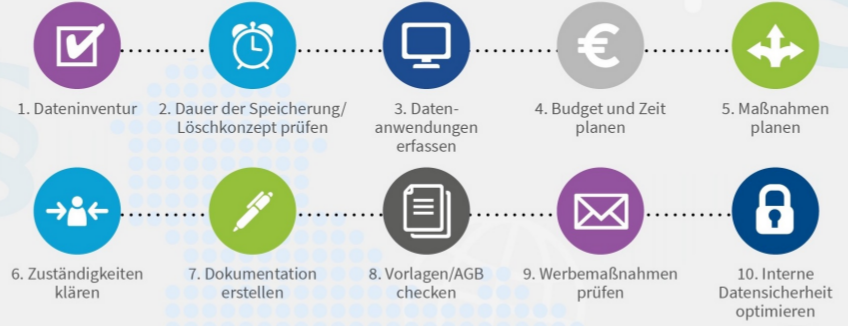
\includegraphics[width=.9\textwidth]{figures/dsgvoSteps.png}
	\caption{Schritte zur DSGVO-Konformität}
\end{figure}

\begin{itemize}
	\tightlist
	\item \textbf{Grundlage jedes Datenschutz-Audits ist die Erhebung des
	aktuellen Zustandes}:\\
	Welche personenbezogenen Daten sind vorhanden? In welcher Form und wo?
	Zu welchem Zweck? Wer zeichnet sich verantwortlich? Wer hat Zugang? Wie
	lange werden diese gespeichert? Handelt es sich um besonders
	schützenswerte Personendaten? Wie werden diese technisch \&
	organisatorisch geschützt? Wie wird das Risiko einer Verletzung \& deren
	Folgen beurteilt?
	\item Die DSGVO verlangt, dass bestehende Verträge (Einwilligungen),
	Datenschutzerklärungen (= Transparenz) und Abläufe angepasst werden. 
	Unternehmen	haben Rechenschaftspflichten (insb. TOMs und Verzeichnis der
	Verarbeitungstätigkeiten).
	\item Bestimmung und Angabe eines Datenschutzbeauftragten (= verantwortlich)
	sowie eines Vertreters in der EU! (= Anlaufstelle für Betroffene und 
	Aufsichtsbehörden für sämtliche	Datenschutzfragen).\\
	(Art. 27 DSGVO)
\end{itemize}

\subsection{DSGVO im Detail}
\begin{description}
	\tightlist
	\item[Ausbau der Rechte der betroffenen Personen] Aufklärungspflichten,
	Transparenz, Zweckbindung, ausdrückliche Einwilligung oder Bezug auf
	Rechtfertigungsgrund. (Art. 5/6 DSGVO).
	\item[Datenhaltung nur solange es der Zweck erfordert] Speicherbegrenzung
	(Art. 5 DSGVO)
	\item[Datenschutz durch Technikgestaltung] Privacy by Design
	(Art. 25 Abs. 1 DSGVO) und datenschutzfreundliche Voreinstellungen/Privacy
	by Default (Art. 25 Abs. 2 DSGVO).
	\item[Big Data] Pflicht zur vorgängigen Durchführung einer
	Datenschutz-Folgenabschätzung (Art. 35 DSGVO).
	\item[Meldepflichten bei Datenschutzverletzungen] an die zuständige
	Aufsichtsbehörde (Art. 33 DSGVO) sowie direkte Benachrichtigung der
	betroffenen Personen bei hohem Risiko von Persönlichkeitsverletzungen.
	\item[Benennung eines Datenschutzbeauftragten]  Bestimmung und Angabe eines
	Datenschutzbeauftragten (= verantwortlich) (Art. 37 DSGVO). Gegebenenfalls
	muss ein Vertreter des Unternehmens in der EU bestimmt werden
	(Art. 27 Abs. 1 DSGVO).
	\item[Auslagerung der Datenverarbeitung](Auftragsverarbeitung) nur auf der
	Grundlage eines Vertrages mit Standardvertragsklausel bei hinreichenden
	Garantien („Datenschutzsiegel“) des Auftragsdatenverarbeiters
	(Art. 28 Abs. 1 DSGVO).
	\item[Recht der betroffenen Person auf Datenübertragbarkeit] in
	strukturierter, maschinenlesbarer Form (Art. 20 DSGVO).
	\item[Keine Unter-Auftragsverarbeitung] (Sub-Sub-Akkordanten) ohne
	schriftliche Genehmigung des Verantwortlichen (Art. 28 Abs. 2 DSGVO).
\end{description}

\section{Digitale Transformation}

Die Digitalisierung verändert vieles. Die Rechnerleistung hat sich in den
letzten Jahren alle zwei Jahre verdoppelt (\textbf{Moor's Law}). Die aktuelle
Technologie stösst jedoch langsam an seine Grenzen. Neue Technologien wie
bspw. Quanten-Computer sind jedoch im Labor-Stadium.

\mbox{}\\
Die rasante Entwicklung hat zu \textbf{Hype Cycles} geführt. An (fast) jede
neu entdeckte Technologie werden Anfangs enorme Erwartungen gestellt.
Nach einer Enttäuschungsphase werden die neuen Technologien dann aber doch
noch entdeckt und marktreif.

\begin{figure}[H]
	\centering
	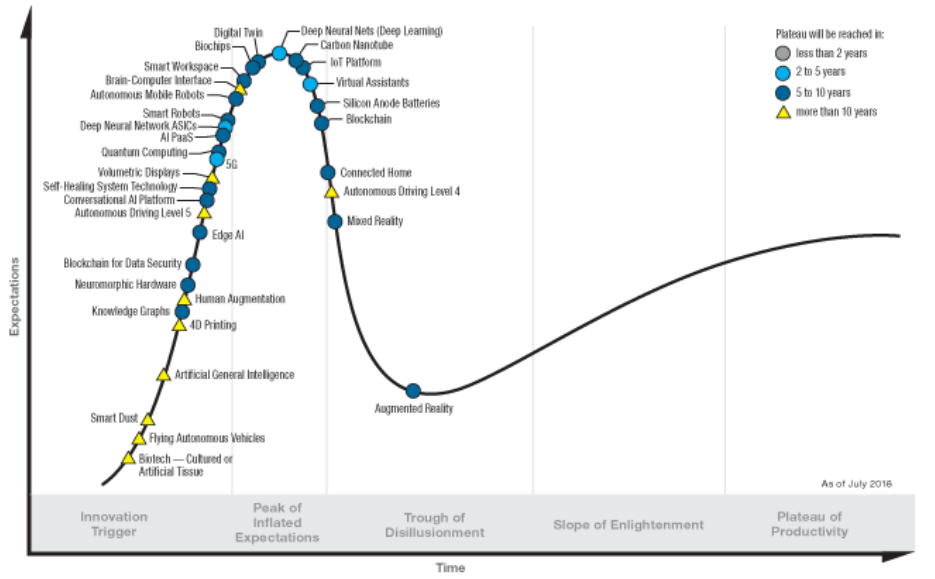
\includegraphics[width=.9\textwidth]{figures/hypeCycle2018.png}
	\caption{Hype Cycle aus dem Jahre 2018}
\end{figure}

\subsection{Digitale Ökonomie}

\begin{itemize}
	\tightlist
	\item Digitale Wirtschaft folgt nicht durchwegs den bisherigen „klassischen“
	ökonomischen Regeln!\\
	z.B. ist der Grenznutzen der Konsumenten bei physischen Gütern relativ rasch
	erreicht - bei	Informationen \& Services dagegen nicht. Daten als
	Ressourcen „verbrauchen“ sich nicht. Sie können immer wieder neu benutzt
	werden.
	\item Geschwindigkeit ist oft wichtiger als Unternehmensgrösse!
	Kleine, agile Unternehmen fordern die Grossen mehr, als umgekehrt.
	\item Oft sind „Markteröffnungs-Strategien“ notwendig (tiefer Preis oder
	kostenlos, limitierte Funktionen, rasches Erarbeiten von Marktanteilen).
	\item Oft rascher Preiszerfall von neuen Produkten oder Dienstleistungen.
	Erwirtschaftung von eigenen Investitionsmittel aus dem Cashflow oft
	schwierig/unmöglich. Viel Fremdkapital = viel Fremdeinfluss...
\end{itemize}

\subsection{Rechtsaspekte der Digitalisierung von Geschäftsprozessen}
\begin{description}
	\tightlist
	\item[EIDI-V] Handhabung von digitalen Rechnungen.
	\item[GeBüV] Aufbewahrungspflichten für digitale Geschäftsakten.
	\item[DSG/DSGVO] Datenschutz/Datensicherheit.
	\item[UWG] Rechtspflichten zur Information von Online-Kunden und
	unlauterer Wettbewerb.
	\item[URG] Urheberrechte
	\item[OR/ArG] Flexibilisierung der Arbeitsverträge
	\item[OR/FusG] Unternehmensreorganisation/Gründungen/Zusammenschluss etc.
\end{description}

\subsubsection{Strafrechtliche Verantwortung}
\label{sec:DigiTrans-Strafrecht}
Die \textbf{ordnungswidrige Führung der Geschäftsbücher}
(Art. 325 StGB) und die \textbf{Unterlassung der Buchführung}
(Art. 166 StGB) werden mit \textbf{Haft, Gefängnis oder mit Busse bestraft.}\\
Für \textbf{strafbare Handlungen im Bereich juristischer Personen}
haften grundsätzlich die tatsächlich \textbf{verantwortlichen
natürlichen Personen}, was für die Delikte der Art. 166 StGB
und Art. 325 StGB ausdrücklich festgelegt wird.

\subsubsection{Haftung der Verwaltung (VR) (Art. 754 OR)}
\label{sec:DigiTrans-VR}

\begin{enumerate}
	\tightlist
	\item Die Mitglieder des Verwaltungsrates und alle mit der Geschäftsführung
	oder mit der Liquidation befassten Personen sind sowohl der Gesellschaft als
	den einzelnen Aktionären und Gesellschaftsgläubigern für den Schaden
	verantwortlich, den sie durch absichtliche oder fahrlässige Verletzung ihrer
	Pflichten verursachen.
	\item Wer die Erfüllung einer Aufgabe befugterweise einem anderen Organ
	überträgt, haftet für den von diesem verursachten Schaden, sofern er nicht
	nachweist, dass er bei der Auswahl, Unterrichtung und Überwachung die nach
	den Umständen gebotene Sorgfalt angewendet hat.
\end{enumerate}

\subsubsection{Aufbewahrungspflichten (Art. 958f OR)}
\label{sec:DigiTrans-Aufbewahrungspflichten}

\begin{enumerate}
	\tightlist
	\item Die Geschäftsbücher und die Buchungsbelege sowie der Geschäftsbericht und der
	Revisionsbericht sind während zehn Jahren aufzubewahren. Die Aufbewahrungsfrist beginnt
	mit dem Ablauf des Geschäftsjahres.
	\item Der Geschäftsbericht und der Revisionsbericht sind schriftlich und unterzeichnet
	aufzubewahren.
	\item Die Geschäftsbücher und die Buchungsbelege können auf Papier, elektronisch oder in
	vergleichbarer Weise aufbewahrt werden, soweit dadurch die Übereinstimmung mit den
	zugrunde liegenden Geschäftsvorfällen und Sachverhalten gewährleistet ist und wenn sie
	jederzeit wieder lesbar gemacht werden können.
\end{enumerate}

\subsubsection{Integrität (Echtheit und Unverfälschbarkeit) (Art. 3 GeBüV)}
\label{sec:DigiTrans-Integrität}
Die Geschäftsbücher müssen so geführt und aufbewahrt und die Buchungsbelege
müssen so erfasst und aufbewahrt werden, dass sie nicht geändert werden können,
ohne dass sich dies feststellen lässt.

\subsubsection{Dokumentationspflichten (Art. 4 GeBüV)}
\label{sec:DigiTrans-Dokumentationspflicht}

\begin{enumerate}
	\tightlist
	\item Je nach Art und Umfang des Geschäfts sind die Organisation, die
	Zuständigkeiten, die Abläufe und Verfahren und die Infrastruktur (Maschinen
	und Programme), die bei der Führung und Aufbewahrung der
	Geschäftsbücher zur Anwendung gekommen sind, in Arbeitsanweisungen so
	zu dokumentieren, dass die Geschäftsbücher und die Buchungsbelege
	verstanden werden können.
	\item Arbeitsanweisungen sind zu aktualisieren und nach den gleichen
	Grundsätzen und gleich lang aufzubewahren wie die Geschäftsbücher,
	die danach geführt wurden.
\end{enumerate}
